\chapter{Field extensions and algebraic curves}

We can sometimes draw pictures of field extensions.
Take an irreducible algebraic curve \(C=(p(x,y)=0)\) in the plane, and look at its field of rational functions \(k(C)\), our favourite example of a field extension of a field \(k\).
\begin{center}
\pgfplotsset{compat=1.12,width=7cm}%
\documentclass{standalone}
\usepackage{tikz}
\usepackage{pgfplots}
\pgfplotsset{compat=1.12,width=7cm}%
\begin{document}
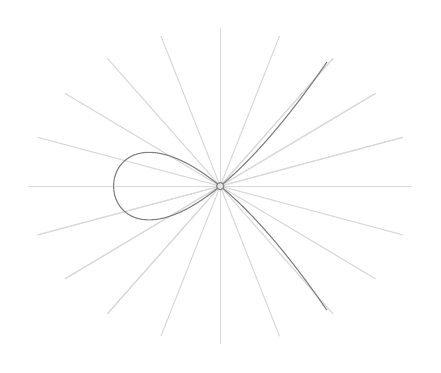
\begin{tikzpicture}
\begin{axis}[hide axis,xmin=-2,xmax=2,ymin=-2,ymax=2]
\newcommand{\RRR}{1.8}
\newcommand{\lineclr}{gray!30}
\draw[\lineclr] 
	({\RRR*cos(3.1415*0/10 r)},{\RRR*sin(3.1415*0/10 r)}) 
-- ({-\RRR*cos(3.1415*0/10 r)},{-\RRR*sin(3.1415*0/10 r)});
\draw[\lineclr] 
	({\RRR*cos(3.1415*1/10 r)},{\RRR*sin(3.1415*1/10 r)}) 
-- ({-\RRR*cos(3.1415*1/10 r)},{-\RRR*sin(3.1415*1/10 r)});
\draw[\lineclr] 
	({\RRR*cos(3.1415*2/10 r)},{\RRR*sin(3.1415*2/10 r)}) 
-- ({-\RRR*cos(3.1415*2/10 r)},{-\RRR*sin(3.1415*2/10 r)});
\draw[\lineclr] 
	({\RRR*cos(3.1415*3/10 r)},{\RRR*sin(3.1415*3/10 r)}) 
-- ({-\RRR*cos(3.1415*3/10 r)},{-\RRR*sin(3.1415*3/10 r)});
\draw[\lineclr] 
	({\RRR*cos(3.1415*4/10 r)},{\RRR*sin(3.1415*4/10 r)}) 
-- ({-\RRR*cos(3.1415*4/10 r)},{-\RRR*sin(3.1415*4/10 r)});
\draw[\lineclr] 
	({\RRR*cos(3.1415*1/10 r)},{-\RRR*sin(3.1415*1/10 r)}) 
-- ({-\RRR*cos(3.1415*1/10 r)},{\RRR*sin(3.1415*1/10 r)});
\draw[\lineclr] 
	({\RRR*cos(3.1415*2/10 r)},{-\RRR*sin(3.1415*2/10 r)}) 
-- ({-\RRR*cos(3.1415*2/10 r)},{\RRR*sin(3.1415*2/10 r)});
\draw[\lineclr] 
	({\RRR*cos(3.1415*3/10 r)},{-\RRR*sin(3.1415*3/10 r)}) 
-- ({-\RRR*cos(3.1415*3/10 r)},{\RRR*sin(3.1415*3/10 r)});
\draw[\lineclr] 
	({\RRR*cos(3.1415*4/10 r)},{-\RRR*sin(3.1415*4/10 r)}) 
-- ({-\RRR*cos(3.1415*4/10 r)},{\RRR*sin(3.1415*4/10 r)});
\draw[\lineclr] 
	({\RRR*cos(3.1415*1/10 r)},{\RRR*sin(3.1415*1/10 r)}) 
-- ({-\RRR*cos(3.1415*1/10 r)},{-\RRR*sin(3.1415*1/10 r)});
\draw[\lineclr] 
	({\RRR*cos(3.1415*2/10 r)},{\RRR*sin(3.1415*2/10 r)}) 
-- ({-\RRR*cos(3.1415*2/10 r)},{-\RRR*sin(3.1415*2/10 r)});
\draw[\lineclr] 
	({\RRR*cos(3.1415*3/10 r)},{\RRR*sin(3.1415*3/10 r)}) 
-- ({-\RRR*cos(3.1415*3/10 r)},{-\RRR*sin(3.1415*3/10 r)});
\draw[\lineclr] 
	(0,\RRR) 
-- (0,{-\RRR});
\newcommand{\curveclr}{gray}
  \addplot[domain=-1:0,\curveclr,samples=200]{sqrt(x^2+x^3)};%
  \addplot[domain=-1:0,\curveclr,samples=200]{-sqrt(x^2+x^3)};%
  \addplot[domain=0:1,\curveclr]{sqrt(x^2+x^3)};%
  \addplot[domain=0:1,\curveclr]{-sqrt(x^2+x^3)};%
  \fill[gray!20,draw=gray] (axis cs:0,0) circle (1.3pt);
\end{axis}
\end{tikzpicture}
\end{document}

\end{center}
Suppose that \(K\) is a field extension of \(k(C)\), say \(K=k(C)(\alpha)\) given by extending by an element \(\alpha\).
We want to draw a curve \(D\) so that \(K=k(D)\).

If \(\alpha\) is transcendental, then \(k(C)(\alpha) \cong k(C)(z)\) for some abstract variable \(z\).
But \(k(C)\) is already a field of rational functions of two variables \(x,y\), quotiented out to enforce the relation \(p(x,y)=0\).
So \(K\) is just the rational functions on the ``cylinder'' \(C \times k\) inside 3-dimensional space, with variables \(x,y,z\); our cylinder has the equation \(p(x,y)=0\), independent of \(z\).
\begin{center}
\includegraphics[width=4cm]{cylinder-on-curve}
\end{center}

Suppose instead that \(\alpha\) is algebraic, say satisfying a polynomial equation \(f(z)=0\) with \(f(z)\) a polynomial with coefficients from \(k(C)\).
So each coefficient of \(f(z)\) is itself a rational function on \(C\).
Each such function is expressible as a rational function of \(x,y\).
Clearing denominators, we get a polynomial equation \(f(x,y,z)=0\) with coefficients in the underlying field \(k\).
The solutions form a surface in 3-dimensional space.
But the resulting surface depends on how we pick out rational functions of \(x,y\) to represent our coefficients of \(f(z)\) from \(k(C)\).
So in fact we have to restrict our \(x,y\) variables to lie in \(C\), i.e. we consider the \emph{curve} \(D\) cut out by the equations \(p(x,y)=f(x,y,z)=0\).
\begin{center}
\includegraphics[width=4cm]{cylinder-on-curve-2}
\end{center}
The map \(\pr{x,y,z} \in D \mapsto \pr{x,y} \in C\) is regular.

We wonder now whether there is a \(k(C)\)-root to \(f(z)=0\), say \(\beta\).
This \(\beta\) is in \(k(C)\), so a rational function on \(C\), so that \(f(\beta)=0\).
So this is a rational map \(z=\beta(x,y)\) from \(C\) to \(D\), lifting the curve \(C\) up from the plane into space, tracing out \(D\) on the cylinder.
In particular, there is no such map if \(D\) is irreducible and \(D \to C\) is many to one:
\begin{center}
\includegraphics[width=4cm]{cylinder-on-curve-3}
\end{center}
So in such a case, \(k(C) \subset k(D)\) is a nontrivial field extension.
We get a picture giving some intuition for nontrivial algebraic field extensions: typically we expect to see an irreducible curve \(D\) mapping to a curve \(C\) by a many-to-one map.

The story continues similarly in higher dimensions: a transcendental extension increases dimension, while an algebraic extension, say of degree \(n\), preserves dimension, giving a new geometric object which maps regularly to the old one, by an \(n\)-to-\(1\) map.

   
\section{Rational curves}

Recall that the \emph{degree}\SubIndex{degree!of field extension} of a field extension \(k \subset K\), denoted \([K:k]\), is the smallest integer \(n\) so that there are \(n\) elements \(\alpha_1, \alpha_2, \dots, \alpha_n\) of \(K\) so that every element of \(K\) is a linear combination \(\sum a_j \alpha_j\) with coefficients \(a_1, a_2, \dots, a_n\) in \(k\).
The degree of the field extension is infinite if there is no such integer \(n\).

\begin{problem}{algebraic.curves:degree.multiplies}
Suppose that \(k \subset K \subset L\) are field extensions.
Prove that \([L:k]=[L:K][K:k]\).
Note: this works even if one or more degree is infinite: let \(n\infty=\infty n = \infty \infty = \infty\) for any positive integer \(n\).
You have to prove these infinite degree cases as well.
\end{problem}

\begin{problem}{algebraic.curves:degree.one}
Prove that a field extension is an isomorphism if and only if it has degree one.
\end{problem}
\begin{answer}{algebraic.curves:degree.one}
Take a basis consisting of one element \(\alpha \in K\).
Then \(1 \in K\) is somehow a multiple \(1=a \alpha\) for some \(a \in k\) so \(\alpha=1/a \in k\).
Any element \(\beta\) of \(K\) is \(\beta=c \alpha\) for some \(c \in k\) so \(\beta \in k\).
\end{answer}

\begin{problem}{algebraic.curves:find.degree}
Suppose that \(p(x)\) is an irreducible polynomial over a field \(k\).
Let \(K\defeq k[x]/(p(x))\).
Prove that \([K:k]\) is the degree of \(p(x)\).
\end{problem}
\begin{answer}{algebraic.curves:find.degree}
Let \(n\) be the degree of \(p(x)\).
We write each element \(b(x)\) in  \(k[x]\) as a polynomial, but if the polynomial has degree \(n\) or more, rewrite it as \(b(x)=q(x)p(x)+r(x)\), quotient and remainder. Then every element of \(K\) is written as the remainder term, i.e. as a polynomial of degree at most \(n-1\).  Hence the elements \(1,x,\dots,x^{n-1}\) in \(k[x]\) map to a spanning set inside \(K\). If not a basis, then there must be some linear relation between them, i.e. a lower degree polynomial in \(x\) vanishing in \(K\), i.e. vanishing modulo \(p(x)\).
But then taking quotient and remainder, we see that this is not possible.
Hence \(K\) has a basis over \(k\) consisting of the images of \(1,x,x^2,\dots,x^{n-1}\) in \(k[x]\).
\end{answer}


\begin{problem}{algebraic.curves:infinitely.many.points.on.trace}
Prove that if \(u(t)\) is a nonconstant rational function over a field \(k\), then there are infinitely many values of \(u(t)\) as \(t\) varies over \(\bar{k}\).
In particular, \(k \subset k(u(t))\) is a transcendental extension.
\end{problem}

Recall that a curve \(C=(0=f(x,y))\) is \emph{irreducible}
\SubIndex{irreducible!polynomial}%
\SubIndex{reducible!polynomial}% 
\SubIndex{polynomial!irreducible}%
\SubIndex{polynomial!reducible}
if \(f(x,y)\) is irreducible.

\begin{theorem}
An irreducible plane algebraic curve \(C\) is rational just when there is a nonconstant rational map \(L \to C\).
In other words, \(C\) is rational just when there are rational functions \(x(t),y(t)\) for which the point \((x(t),y(t))\) lies in \(C\) for all \(t\) in the algebraic closure of the field.
\end{theorem}
\begin{proof}
If our curve \(C\) is rational then by definition \(C\) is birational to a line, so there is such a map.
Suppose on the other hand that there is such a map \(L \to C\), say written as \(t \in L \mapsto (x(t),y(t)) \in C\) with
\[
f(x(t),y(t))=0
\]
for some rational functions \(x(t), y(t)\), not both constant.
As we vary \(t\) through \(\bar{k}\), the moving point \((x(t),y(t))\) moves through infinitely many different points of the plane.
Take a rational function on \(C\), say \(g(x,y)=b(x,y)/c(x,y)\).
Then \(c(x,y)\ne 0\) at all but finitely points of \(C\).
(Note that this requires that our curve \(C\) is irreducible, as otherwise we might have \(g(x,y)\) vanishing on a component of \(C\).)
So at infinitely many values of \(t\), \(g(x(t),y(t))\) is defined.
We map \(g(x,y) \in k(X) \mapsto g(x(t),y(t)) \in k(t)\), a morphism of fields. 
The image is some subfield \(K=k(x(t),y(t)) \subset k(t)\).
The result follows from the following theorem applied to \(K\).
\end{proof}

\begin{theorem}[L\"uroth's theorem]\define{Luroth's theorem@L\"uroth's theorem}\define{theorem!Luroth@L\"uroth}
Suppose that \(k \subset K \subset k(t)\) is a finitely generated extension of a field \(k\), where \(t\) is an abstract variable.
Then \(K=k(f(t))\) is generated by a single rational function \(f(t)\) in \(k(t)\).
In particular, either \(K=k\) (if \(f(t)\) is a constant function) or \(K\) is isomorphic to \(k(t)\) by \(t \mapsto f(t)\).
\end{theorem}
The proof of this theorem requires a lemma:
\begin{lemma}
Take a nonconstant rational function \(f(x)=b(x)/c(x)\), with \(b(x), c(x)\) coprime, over a field \(k\).
Then, as a polynomial in a variable \(y\) with coefficients in \(k(f(x))\), the expression
\[
f(x)c(y)-b(y) 
\]
in \(k(f(x))[y]\) is irreducible.
\end{lemma}
\begin{proof}
This expression is not zero, because it is nonconstant in \(x\).
It vanishes at \(y=x\).
Hence \(x\) satisfies this polynomial (in \(y\)) expression with coefficients in \(k(f(x))\).
So \(k(x)\) is an algebraic extension of \(k(f(x))\).
Since \(k(x)\) is transcendental over \(k\), \(k(f(x))\) is transcendental over \(k\).
So \(f(x)\) solves no polynomial equation over \(k\).
Take an abstract variable \(t\). 
Map \(k(t,y) \to k(f(x),y)\) by \(t \mapsto f(x)\).
This map is an isomorphism of fields.
Similarly \(k[t,y] \to k[f(x),y]\) is an isomorphism of rings.
In order to prove that \(tc(y)-b(y)\) is irreducible in \(k(t)[y]\), it suffices to prove that it is irreducible in \(k[t,y]\), i.e. clear \(t\) from denominators, by Gauss's lemma (proposition~\vref{proposition:Gauss.lemma}).
If we can factor \(tc(y)-b(y)=g(t,y)h(t,y)\) in \(k[t,y]\) then one of \(g(t,y)\) or \(h(t,y)\) has degree \(1\) in \(t\), since the product does, and so one of \(g(t,y)\) or \(h(t,y)\) has degree zero in \(t\), depending only on \(y\), say \(g(t,y)=g(y)\).
Then \(g(t)h(t,y)=tc(y)-b(y)\), so \(g(y)\) divides \(tc(y)-b(y)\), and since \(t\) is an abstract variable, \(g(y)\) divides \(b(y)\) and \(c(y)\), which are coprime, so \(g(y)\) is a nonzero constant.
\end{proof}

We now prove L\"uroth's theorem:
\begin{proof}
For each element \(f(t)=b(t)/c(t)\) in \(K\), let \(n\) be the  larger of the degrees of \(b(t),c(t)\).
Pick an element \(f(t)=b(t)/c(t)\) in \(K\), not in \(k\), for which the value of \(n\) is as small as possible.
By the previous lemma, the polynomial \(B(y)=f(x)c(y)-b(y)\) is irreducible in \(k(f(x))[y]\), so the map
\[
x,y \in k(f(x))[y]/(B(y)) \mapsto x,x \in k(x)
\]
is an isomorphism of fields and \([k(x):k(f(x))]=n\).
The expression \(B(y)\) is the polynomial in \(K[y]\) of smallest positive \(y\)-degree which is satisfied by \(y=x\), since a smaller degree one would give a smaller value for \(n\).
Indeed the \(y\)-degree of \(B(y)\) is \(n\).
In particular, \(B(y)\) is also irreducible in \(K[y]\) and the map
\[
x,y \in K[y]/(B(y)) \mapsto x,x \in k(x)
\]
is an isomorphism.
In particular, \([k(x):K]=n\).
But
\begin{align*}
n
&=[k(x):k(f(x))],
\\
&=[k(x):K][K:k(f(x))],
\\
&=n[K:k(f(x))]
\end{align*}
so \([K:k(f(x))]=1\).
\end{proof}
   
   